%%%%%%%%%%%%%%%%%%%%%%%%%%%%%%%%%%%%%%%%%%%%%%%%%%%%%%%%%%%%%%%%%%%%%%%%%%%
%% This file is part of the book
%%
%% Algorithmic Graph Theory
%% http://code.google.com/p/graph-theory-algorithms-book/
%%
%% Copyright (C) 2009, 2010 Minh Van Nguyen <nguyenminh2@gmail.com>
%%
%% See the file COPYING for copying conditions.
%%%%%%%%%%%%%%%%%%%%%%%%%%%%%%%%%%%%%%%%%%%%%%%%%%%%%%%%%%%%%%%%%%%%%%%%%%%

%% sin(x) and coordinates
\subfigure[Plots of functions.]{
\begin{tikzpicture}[scale=0.85]
\begin{axis}[
    xlabel=$x$,%
    ylabel=$f(x)$
  ]
%% invoke external gnuplot as calculator
\addplot[smooth,color=blue] gnuplot{sin(x)};
\addplot[smooth,color=red] gnuplot{cos(x)};
\end{axis}
\end{tikzpicture}
}
\quad
%%
%% scatterplot
\subfigure[A scatterplot.]{
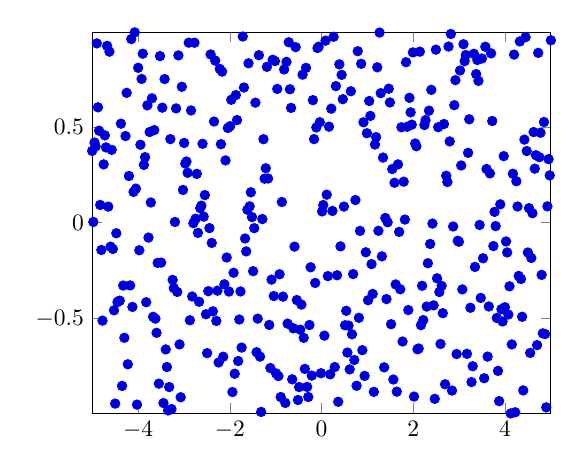
\begin{tikzpicture}[scale=0.85]
\begin{axis}[enlargelimits=false]
\addplot+[only marks,samples=400] {rand};
\end{axis}
\end{tikzpicture}
}
